%%%%%%%%%%%%%%%%%%%%%%% file template.tex %%%%%%%%%%%%%%%%%%%%%%%%%
%
% This is a general template file for the LaTeX package SVJour3
% for Springer journals.          Springer Heidelberg 2010/09/16
%
% Copy it to a new file with a new name and use it as the basis
% for your article. Delete % signs as needed.
%
% This template includes a few options for different layouts and
% content for various journals. Please consult a previous issue of
% your journal as needed.
%
%%%%%%%%%%%%%%%%%%%%%%%%%%%%%%%%%%%%%%%%%%%%%%%%%%%%%%%%%%%%%%%%%%%
%
% First comes an example EPS file -- just ignore it and
% proceed on the \documentclass line
% your LaTeX will extract the file if required
\begin{filecontents*}{example.eps}
%!PS-Adobe-3.0 EPSF-3.0
%%BoundingBox: 19 19 221 221
%%CreationDate: Mon Sep 29 1997
%%Creator: programmed by hand (JK)
%%EndComments
gsave
newpath
  20 20 moveto
  20 220 lineto
  220 220 lineto
  220 20 lineto
closepath
2 setlinewidth
gsave
  .4 setgray fill
grestore
stroke
grestore
\end{filecontents*}
%
\RequirePackage{fix-cm}
%
%\documentclass{svjour3}                     % onecolumn (standard format)
%\documentclass[smallcondensed]{svjour3}     % onecolumn (ditto)
%\documentclass[smallextended]{svjour3}       % onecolumn (second format)
\documentclass[twocolumn]{svjour3}          % twocolumn
%
\smartqed  % flush right qed marks, e.g. at end of proof
%

%
\usepackage{mathptmx}      % use Times fonts if available on your TeX system
%
% insert here the call for the packages your document requires
%\usepackage{latexsym}
\usepackage[demo]{graphicx}
\usepackage[caption = false]{subfig}
\graphicspath{ {./images/} }
\usepackage[round]{natbib}
\usepackage{amsmath}  
\usepackage{amsfonts} 
\usepackage{graphicx} 
\usepackage[usenames]{color}
\usepackage{mathtools}
\usepackage{algorithm}
\usepackage[noend]{algpseudocode}
\usepackage{float}

% etc.
%
% please place your own definitions here and don't use \def but
% \newcommand{}{}
\newcommand{\Real}{\mathbb R}
\newcommand{\E}{\mathbb{E}}
\newcommand{\s}{\mathbb{S}}
\renewcommand{\P}{\mathbb{P}}
\newcommand{\K}{\mathbb{K}}
\newcommand{\Q}{\mathbb{Q}}
\newcommand{\eps}{\varepsilon}
\newcommand{\diag}{\mathrm{diag}}
\newcommand{\nbr}{\mathrm{nbr}}
\newcommand{\F}{\mathcal{F}}
\newcommand{\Qm}{\mathcal{Q}}
\newcommand{\M}{\mathcal{M}}
\newcommand{\Z}{\mathcal{Z}}
\newcommand{\csimplex}{\bar{\mathcal{S}}^{d-1}}
\newcommand{\osimplex}{\mathcal{S}^{d-1}}
\newcommand{\LL}{\mathcal{L}}
\newcommand{\Hil}{\mathscr{H}}
\newcommand{\G}{\mathscr{G}}
\newcommand{\p}{\mathscr{P}}
\newcommand{\C}{\mathscr{C}}
\newcommand{\one}[1]{\mathbf{1}_{\{#1\}}}
\newcommand{\oneset}[1]{\mathbf{1}_{#1}}
\newcommand{\argmin}{\mathrm{argmin}}
\newcommand{\argmax}{\mathrm{argmax}}
\newcommand{\var}{\mathrm{Var}}
\newcommand{\cov}{\mathrm{Cov}}
\newcommand{\ind}{\mathrm{I}}
\newcommand{\D}{\mathrm{d}}
\newcommand{\Borel}{\mathscr{B}}
\newcommand{\ben}{\begin{enumerate}}
\newcommand{\een}{\end{enumerate}}
\newcommand{\ds}{\displaystyle}
\newcommand{\voila}{\hfill $\blacksquare$}
\newcommand{\Id}{\mathrm{Id}}
\renewcommand{\Re}{\mathrm{Re}}
\renewcommand{\vec}[1]{\mathbf{#1}}
\renewcommand{\d}[1]{\ensuremath{\operatorname{d}\!{#1}}}
\newcommand*\diff{\mathop{}\!\mathrm{d}}

\DeclareMathOperator{\esssupp}{ess\,supp}
%
% Insert the name of "your journal" with
\journalname{Statistics and Computing}
%
\begin{document} \sloppy
\bibliographystyle{plainnat}

\title{Sequential Importance Sampling With Corrections For Partially Observed States
%\thanks{Grants or other notes
%about the article that should go on the front page should be
%placed here. General acknowledgments should be placed at the end of the article.}
}

%\titlerunning{Short form of title}        % if too long for running head

\author{Valentina Di Marco         \and
        Jonathan Keith \and
        Daniel Spring
}

%\authorrunning{Short form of author list} % if too long for running head

\institute{Valentina Di Marco \at
              School of Mathematical Science, Monash University, Clayton Campus, VIC 3800, Australia \\
              Tel.: +61-4-23330509\\
              \email{valentina.dimarco@monash.edu}           %  \\
%             \emph{Present address:} of F. Author  %  if needed
           \and
           Jonathan Keith \at
              School of Mathematical Science, Monash University, Clayton Campus, VIC 3800, Australia
	   \and
	  Daniel Spring \at
	      School of Ecosystem and Forest Sciences, The University of Melbourne, Parkville, Victoria 3010, Australia
}

\date{Received: date / Accepted: date}
% The correct dates will be entered by the editor


\maketitle

\begin{abstract}

We consider an evolving system for which a sequence of observations is being made, with each observation revealing additional information about current and past states of the system. We suppose each observation is made without error, but does not fully determine the state of the system at the time it is made. Our motivating example is drawn from invasive species biology, where it is common to know the precise location of invasive organisms that have been detected by a surveillance program, but at any time during the program there are invaders that have not been detected.

We propose a sequential importance sampling strategy to infer the state of the invasion under a Bayesian model of such a system. The strategy involves simulating multiple alternative states consistent with current knowledge of the system, as revealed by the observations. However, a difficult problem that arises is that observations made at a later time are invariably incompatible with previously simulated states.

To solve this problem, we propose a two-step iterative process in which states of the system are alternately simulated in accordance with past observations, then corrected in light of new observations. We identify criteria under which such corrections can be made while maintaining appropriate importance weights.

\keywords{ Sequential Importance Sampling \and Filtering \and Bayesian estimation \and Partially observed spaces \and Missing data}
% \PACS{PACS code1 \and PACS code2 \and more}
% \subclass{MSC code1 \and MSC code2 \and more}
\end{abstract}

\section{Introduction}
This paper considers the problem of imputing missing data in the presence of incomplete observations made sequentially in real time. We thus envisage data that consists of a series of correlated observations made sequentially in time, each of which is correct but only partially reveals the true state of the system. The main difficulty that arises in this context is that data missing at one time point can be revealed at a later time point, so that imputed missing values must later be corrected in light of new information.

Our original motivation for considering this problem was to facilitate analysis of the Red Imported Fire Ant (RIFA) invasion in Queensland, Australia, where in an ongoing surveillance program, the locations of ants’ nests are regularly being detected. For detected nests, the location can be precisely determined, but at any given time there is an unknown number of undetected nests, each with an unknown location. To infer the current extent of the invasion, we aim to impute plausible locations of undetected individuals, but these imputations are only informed guesses, and will require constant correction as new detections come to light.

In addition, new nests are constantly being produced: the unseen state of the system is thus constantly evolving. Knowing the location of at least some of the invaders at time $t$, we can simulate the evolution of this system. However, again the imputed locations of simulated nests will require constant correction as more information about the true state of the system becomes available.

In this paper, we propose a new approach to problems of this type. Although our approach is ultimately aimed at inference for invasive species, here we will illustrate the method for less complex evolving systems in which correct but partial observations are being made in real time.

To handle problems of this kind, we introduce a Bayesian approach that uses a new sequential importance sampling (SIS) strategy. As is typical of SIS methods, we generate a population of particles, each representing a plausible sequence of system states, and we evolve each particle at each time step according to a model of system dynamics. Again in a manner typical of SIS methods, new observations arrive in real time, and we use these observations to adjust the weights assigned to particles. However, a crucial new element in our method is that we allow missing values imputed at earlier time steps to be corrected so that they are consistent with the new observations.

Our method thus addresses a problem that is common in practice: new observations made in real time can render previously imputed missing values implausible, and may even conflict with what has been simulated. For example, in the invasive species context described above, undetected nests imputed to geographic areas that do not contain any nests become increasingly implausible as time passes without detections being made in those regions. In standard SIS approaches, such particles receive low weights and are eventually eliminated by resampling, but a common problem is that all particles can become implausible, if not inconsistent, with observations.

Problems of this kind arise in many contexts. We can envisage the approach being used to study the evolution of a species' geographic range, for both invasive and non-invasive species. The algorithm could be also applied to a variety of other missing data problems where new incomplete data is continuously acquired, like in crime prediction, (\cite{Malathy}) or bushfire modeling (\cite{Beer}). Another potential application is in the study of the spread of infectious diseases, where observations are made in the form of diagnosed cases, but missing data in the form of undiagnosed cases is unavoidable (\cite{O'Neill}). 

Missing data are ubiquitous in ecological and evolutionary data sets as in any other branch of science. The common methods used to deal with missing data are to delete cases containing missing data, and to use the mean to fill in missing values. However, these ‘traditional’ methods result in biased estimation of parameters and uncertainty, and reduction in statistical power. Better missing data procedures such as data augmentation (\cite{Tanner}) and multiple imputation (\cite{RubinMI}) are readily available and implementable (\cite{Nakagawa}).

Particle filters are used to estimate a hidden state when partial (noisy) observations are made. However, the standard particle filtering algorithm can diverge or its performance can severely degrade in the presence of missing data (\cite{Zhang}).

On the other hand, multiple imputations do not use past observations and the state transition equations when estimating the probability of the hidden state knowing the observations. This can result in poor performance when the problem can be well modelled by a Markov structure (\cite{Zhang}).

In the context of missing observations, \cite{Zhang} have developed a Multiple Imputation Particle Filter (MIPF) to deal with these deficiencies. This method uses randomly drawn values (imputations) to provide a replacement for the missing data and then uses the particle filter to estimate non-linear state with the data.

Data Augmentation methods in Bayesian statistic are normally used to evaluate an intractable posterior distribution of the parameters when data can be augmented in such a way that it become easy to analyse the augmented data (\cite{Tanner}).

In our method we will use data augmentation in sequential importance sampling in order to simulate the new state of the system using a first set of samples and a second sample corrected in light of new data acquired at each step.

Our method deals with situations where the data are informative, a situation where standard sequential Monte Carlo methods can perform poorly. 

Similarly, \cite{Del Moral} have proposed a Sequential Monte Carlo method for sampling the posterior distribution of state-space models under highly informative observation regimes. In their method they introduce a schedule of intermediate weighting and resampling times between observation times, which guide particles towards the final state.

A similar method was used by Finke et al. (2018) who developed a Particle Monte Carlo Markov Chain algorithm to estimate the demographic parameters of a population and then incorporated this algorithm into a sequential Monte Carlo sampler in order to perform model comparison motivated by the fact that a simple importance sampling performs poorly if there is a strong mismatch between the prior and the posterior, which is common when the data is highly informative.

In this paper we provide a proof of concept for our proposed methodology using a simple system modelled by an AR(1) process. Here we present a version of our method in which only those imputed values that are strictly inconsistent with later observations are corrected, in a deterministic manner. We also envisage the possibility of generalising this approach to allow \\ non-deterministic revision of imputed values that, while not inconsistent with later observations, can nevertheless be updated in light of new information.

(HHH to be finalised: In chapter 1 we introduce the method ...
In chapter 2 we apply the methodology to a simple stationary AR(1) model...
In chapter 3 we apply the methodology to a river invasion...
In chapter 4 we apply the methodology to the dataset...
Chapter 5 contains the conclusions of our article.)

\section{The Sequential Importance Sampling with corrections approach}

In our present applications we will consider a system or an invasion that will evolve discretely in time. The state of this system at time $t$ will be represented by a vector $\vec{x}^t = x^t_1, \dots, x^t_M$ and the full evolution of the system up to a certain time $\tau$ will therefore be defined by a matrix $\vec{X}^{\tau} = (\vec{x}^1, \dots, \vec{x}^{\tau})$ on a topological measure space $(\Omega_x, \F_x, \lambda_x)$ where $\Omega_x = \prod_{i=1}^M (\Omega_x)_i$ and $(\Omega_x)_i \subseteq \Real^t$. Partial observations $\vec{Z}^t = (\vec{z}^t_1, \dots, \vec{z}^t_M)$ with $\vec{z} = z_1, \dots, z_M$ are made on a second topological measure space $(\Omega_z, \F_z, \lambda_z)$ where $\Omega_z = \prod_{i=1}^M (\Omega_z)_i$ and $(\Omega_z)_i \subseteq \Real^t$. The processes $\vec{x}^t$ and $\vec{z}^t$ will be independent, meaning that the act of observing does not influence the growth of the system and vice-versa. 

Since not not all the elements of $\vec{X}^{\tau}$ will be observed at each time $t$, our matrix $\vec{Z}^{\tau}$ will have some elements that are dashes (-), or zeroes if zero is not a legitimate observation of the system. Those dashes represent the elements that we don't observe. On the other hand we consider our observations to be exact, therefore each element of $\vec{Z}^{\tau}$ that is not a dash will completely define the value of $x^t_s$ in position $s$ at that time $t$, so if $z^t_s \neq -$ then $x^t_s = z^t_s$. Notice that once an element of $\vec{X}^t$ have been observed, it will remain observed for all subsequent times. The elements of $\vec{X}^t$ that are not observed will have to be simulated at each time.

In order to do so we will define a sequential importance sampling strategy to simulate the posterior distribution $p(\vec{x}^t | \vec{Z}^t)$ at each step knowing the distribution $q(\vec{X}^t, \vec{Z}^t | \vec{Z}^t)$ that represent the knowledge we have of the system before we observe $\vec{Z}^t$
We will have a prior distribution $q$ defined on the subspace $\Omega = \Omega_x \times \Omega_z$ that will represent our knowledge of the system before we make the next set of observations $\vec{z}^t$

Also our system will be such that each step of the evolution will depend only on the previous step, meaning that at each time $t$ the vector $\vec{x}^t$ will only depend on the vector $\vec{x}^{t-1}$ following a certain state transitional density distribution $f$. We will also have that the observations will depend on the current state and on the observations at the previous time following a certain distribution $g$.
\begin{align*}
    &\vec{x}^t | \vec{x}^{t-1} \sim f(\vec{x}^t | \vec{x}^{t-1})\\
    &\vec{z}^t | \vec{x}^t, \vec{z}^{t-1} \sim g(\vec{z}^t | \vec{x}^t, \vec{z}^{t-1}).
\end{align*}

Our goal will be to determine the posterior distribution of the state of the system in light of the observations via a sampling process.

In order to do so in our partially observed system, we use Bayes theorem on the posterior
This means that we will be able to write the posterior $p$ as follow
\begin{equation*}
    p(\vec{X}^t, \vec{Z}^t | \vec{Z}^t) =
\end{equation*}

Our goal will be to determine the posterior distribution of the state of the system in light of the observations via a sampling process.

In order to do so in our partially observed system, we use Bayes theorem on the posterior

At each time $t$ we will observe some elements of the system and these observations at each time $t$ will be represented by a vector $\vec{z}^t$. It follows that only some elements $x^t_s$ of the vector $\vec{x}^t$ will be observed and will coincide with the corresponding non zero elements of $\vec{z}^t$, $z^t_s$ . 

We will want to estimate the evolution of the system in light of all the available observations at the current time $\tau$, therefore estimate the distribution $p(\vec{X}^{\tau} | \vec{Z}^{\tau})$ where $\vec{X}^{\tau} = \vec{x}^1, \dots \vec{x}^\tau$ and $\vec{Z}^{\tau} = \vec{z}^1, \dots \vec{z}^\tau$.


The state space is a topological measure space $(\Omega, \F, \lambda)$ on which a prior probability measure $\Q$ having density $q(\vec{x}^t)$ relative to the Borel measure $\lambda$ has been defined. Partial observations are made in a second topological measure space $(\Omega', \F', \lambda')$ such that there is a measurable function $\sigma : \Omega \rightarrow \Omega'$ with $\lambda' = \lambda \circ \sigma^{-1}$. Thus $\sigma$ projects $\Omega$ onto $\Omega'$, and only the projection is observed. A partial observation $\vec{z}^t \in \Omega'$ fixes the value $\sigma(\vec{x}^t) = \vec{z}^t$, or equivalently, it consists of information that the system is in some state $x \in \sigma^{-1} (\vec{z}^t)$.

This scenario is more general than at first appears. A more common circumstance in Bayesian inference is that a state $x \in \Omega$ determines a conditional probability measure $\P(\cdot|x)$ over the observation space $\Omega'$, rather than a specific element $\sigma(x)$. However, we may define an augmented space $\Omega^* = \Omega' \times \Omega$ and then define a projection $\sigma : \Omega^* \rightarrow \Omega'$ by $\sigma(x, z) = z$. Thus the partially observed state space framework subsumes the more common circumstance as a special case.

We want to determine the posterior distribution for $x$ in light of the observation $z$. Intuitively, this is just the prior $q(x)$ re-normalised over $\sigma^{-1}(z)$. More formally use the disintegration theorem to obtain a family of measures $\{ \mu_z \}_{z \in \Omega'}$ on $\Omega$ such that for every Borel measurable function $l : \Omega \rightarrow [0, \infty]$ 

\begin{equation*}
    \int_\Omega l(x) \D \lambda(x) = \int_{\Omega'}\int_{\sigma^{-1}(z)} l(x) \D \mu_z (x) \D \lambda' (z).
\end{equation*}
Then the posterior distribution of $x$ in light of the observation $z$ has a density with respect to $\mu_z$ given by

\begin{equation*}
    p(\vec{x}^t|\vec{z}^t) \propto 
    \begin{cases}
        q(\vec{x}^t), & \vec{x}^t \in \sigma^{-1}(\vec{x}^t)\\
        0, & \mbox{otherwise}
    \end{cases}
\end{equation*}
with constant of proportionality $r(z)^{-1}$ where

\begin{equation*}
    r(z) = \int_{\sigma^{-1}(z)} q(x) \D \mu_z(x).
\end{equation*}
Note that $r(z)$ is the density of the pushforward measure $\Q \circ \sigma{-1}$ with respect to $\lambda'$.

Importance sampling is a form of Monte Carlo integration in which one uses a sample drawn from one probability distribution in order to estimate an expectation with respect to a second probability distribution. Consider a topological measure space $(\Omega, \F, \lambda)$ where $\lambda$ is a Borel measure and $\Omega \subset \Real^n$ and consider two probability measures $\P$ and $\Q$ having densities $p$ and $q$ with respect to $\lambda$. Let $h : \Omega \rightarrow \Real$ be a function for which we want to estimate and expectation under $\P$. The idea of importance sampling is to draw and iid sample $\vec{x}_1 , \dots, \vec{x}_n \in \Omega$ distributed according to $\Q$, then approximate the expectation as follows:
\begin{align*}
    E_{\P}[h(\vec{x})] &= \int_{\Omega} h(\vec{x})p(\vec{x})\D\lambda(\vec{x})\\
    &= \int_{\Omega} h(\vec{x})\frac{p(\vec{x})}{q(\vec{x})}q(\vec{x})\D\lambda(\vec{x})\\
    &\approx \sum_{i=1}^n h(\vec{x}_i) w_i
\end{align*}
where the second integral is over $\Qm = \esssupp (q)$ and the terms 
\begin{equation*}
    w_i = \frac{p(\vec{x}_i)}{q(\vec{x}_i)}\Bigg ( \sum_{i=1}^n \frac{p(\vec{x}_i)}{q(\vec{x}_i)}\Bigg)
\end{equation*}
for $i = 1, \dots, n$ are referred to as \emph{sample weights}. Note that importance sampling is appropriate only if $\esssupp(p) \subseteq \Qm$.

Importance sampling may be useful when it is easier to sample from the importance density $\Q$ than $\P$, or when the resulting estimate has lower variance than the direct Monte Carlo estimate based on sampling $\P$. Ideally, $p$ and $q$ should have the same essential support so that importance weights are never zero.

\subsection{Importance Sampling with an auxiliary variable}

Here we propose to introduce an auxiliary variable to importance sampling. This will allow us to simulate sampling via a two-step process in which we generate a first sample $\vec{x_1}, \dots, \vec{x_n}$ (the auxiliary variable) then correct in light of data to obtain $\vec{x'_1}, \dots, \vec{x'_n}$. We will interpret the term "auxiliary variable" in a broad sense, using a projection map to relate the augmented state space to the original state space. Consider two topological measure space $(\Omega_1, \F_1, \lambda_1)$ and $(\Omega_2, \F_2, \lambda_2)$, where $\lambda_1$ and $\lambda_2$ are Borel measures, and a measurable function $\pi: \Omega_2 \rightarrow \Omega_1$ such that $\lambda_1 = \lambda_2 \circ \pi^{-1}$. Here $\Omega_2$ is the augmented state space and $\pi$ is a projection of this space onto the original state space $\Omega_1$. We want to estimate the expectation of a function $f:\Omega_1 \rightarrow \Real$ with respect to a probability measure $\P$ on $\Omega_1$ having density $p$ with respect to $\lambda_1$. We have at our disposal a method of sampling from a distribution with measure $\Q$ on $\Omega_2$ having density $q(\vec{x', \vec{x}}) > 0$ with respect to $\lambda_2$. Our strategy is to define a measure $\P^*$ on $\Omega_2$ having density $p^*(\vec{x}', \vec{x})$ with respect to $\lambda_2$, such that the marginal distribution of $\P^*$ on $\Omega_1$ is $\P$, that is $\P = \P^* \circ \pi^{-1}$. We also need to ensure that $\esssupp(p^*) \subseteq \esssupp(q)$, so that we can apply importance sampling.
By the disintegration theorem there exists a family of measure $\{ \nu_{\vec{x}} \}_{\vec{x}\in\Omega_1}$ on $\Omega_2$ such that for every Borel measurable function $l:\Omega_2 \rightarrow [0, \infty]$:
\begin{equation*}
    \int_{\Omega_2} l(\vec{x'}, \vec{x}) \d \lambda_2(\vec{x'}, \vec{x}) = \int_{\Omega_1}\int_{\pi^{-1}} l(\vec{x', \vec{x}}) \d \nu_\vec{x}(\vec{x', \vec{x}}) \D \lambda_1(\vec{x}).
\end{equation*}
It follows that for any $A \in \F_1,$
\begin{align*}
    \P(A) &= \P^*(\pi^{-1}(A)) = \int_{\Omega_2} I_A(\pi(\vec{x', \vec{x}}))p^*(\vec{x', \vec{x}})\D \lambda_2(\vec{x', \vec{x}}) \\
    &= \int_{\Omega_1} I_A(\vec{x})\Bigg[\int_{\pi^{-1}(\vec{x})}p^*(\vec{x', \vec{x}})\d \nu(\vec{x', \vec{x}}) \Bigg] \D \lambda_1(\vec{x})
\end{align*}
and hence $p(\vec{x}) = \int_{\pi^{-1}(\vec{x})}p^*(\vec{x',\vec{x}})\d \nu_{\vec{x}}(\vec{x', \vec{x}})$. Moreover,
\begin{align*}
    E_{\P^*}[h(\pi(\vec{x', \vec{x}}))] &= \int_{\Omega_2}f(\pi(\vec{x', \vec{x}}))p^*(\vec{x', \vec{x}})\D \lambda_2(\vec{x', \vec{x}})\\
    &= \int_{\Omega_1} h(\vec{x}) \Bigg[ \int_{\pi^{-1}(\vec{x})} p^*(\vec{x'}) \D \nu_{\vec{x}}(\vec{x', \vec{x}}) \Bigg] \D \lambda_1 (\vec{x})\\
    &= \int_{\Omega_1} h(\vec{x}) p(\vec{x}) \D \lambda_1 (\vec{x}) \\
    &= E_{\P}[f(\vec{x})].
\end{align*}
Now using importance sampling in $\Omega_2$, we obtain:
\begin{equation*}
    E_{\P^*}[f(\vec{x})] = E_{\P^*}[f(\pi (\vec{x',\vec{x}}))] \approx \sum_{i=0}^{n} f(\pi ((\vec{x'}, \vec{x})_i)) w_i
\end{equation*}
were the sample weights are 
\begin{equation*}
    w_i = \frac{p'((\vec{x'}, \vec{x})_i)}{q((\vec{x'}, \vec{x})_i)} = \Bigg( \sum_{i=1}^n \frac{p'((\vec{x'}, \vec{x})_i)}{q((\vec{x'}, \vec{x})_i)} \Bigg)^{-1}
\end{equation*}
for $i = 1, \dots, n$.

Since our corrections are deterministic, $\vec{x'} \in \Omega$ is a deterministic function of $\vec{x}$. We treat $\vec{x'}$ as an auxiliary variable: the augmented space is $\Omega_{\vec{z}} = \{(\vec{x'}, \vec{x}) : \vec{x'} \in \Omega, \vec{x} \in \sigma^{-1}(\vec{Z}) \} $. Measurable sets in $\Omega_z$ are of the form {}






\section{Application to a stationary AR(1) model}

Let us first introduce our importance sampling idea using a simple example.

Consider a linear, normal and stationary AR(1) process for which
\begin{equation*}
    x_{t} = \varphi x_{t-1} + \eps_{t}
\end{equation*}
with $\eps_{t} \stackrel{iid}{\sim} \mathcal{N}(0, \sigma^{2})$.
Then
\[
    (x_{t} | x_{t-1}) \sim \mathcal{N} (\varphi x_{t-1}, \sigma^{2}).
\]
This process is stationary provided that the initial distribution is
\[
x_{1} \sim \mathcal{N} \Bigg (0, \frac{\sigma^2}{1- \varphi^2} \Bigg )
\]
which is valid only if $|\varphi| < 1$.

Suppose that at any time $t$, only some subset of the values $\vec {x}^{t} = (x_1, \dots, x_{t})$ have so far been observed. However, those that have been observed are known without error. We collect the values that have been observed at or before time $t$ to form a vector $\vec{z}^{t} = (z_1^{t}, \dots, z_{t}^{t})$, where for each $s \leq t$, $z_s^{t} = x_s$ if $x_s$ has been observed at or before time $t$ and $z_s^{t} = -$ otherwise. Thus the coordinates of $\vec{z}^{t}$ belong to an extension of the reals $\mathbb{R} \cup \{ - \}$.

As time progresses, new observations become available. Thus some dashes in the vector $\vec{z}^{t}$ will be replaced by observations in the subsequent vector $\vec{z}^{t+1}$. However, the reverse does not occur: if we have $z_s^{t} = x_s$ for times $s$ and $t$ where $s \leq t$ then we must also have $z_s^{t^{\prime}} = x_s$ at all subsequent times $t^{\prime} > t$.

We will therefore define a lower triangular $t \times t$ matrix $\vec{Z}^{t}$ in which row $i$ is the vector $\vec{z}^{i}$.

In this example will also define binary vectors $\vec{b}^{t} = (b_1^{t}, \dots, b_{t}^{t})$, where $b_s^{t} = 1$ if $z_s^{t} = x_s$, and $b_s^{t} = 0$ if $z_s^{t} = -$, and a lower triangular $t \times t$ binary matrix $\vec{B}^{t}$ in which row $i$ is the vector $\vec{b}^{i}$.
The matrix $\vec{B}^{t}$ must satisfy the constraints that if $B_{ij}^{t} = b_j^{i} = 1$ for $i \in \{ 1, \ldots, t \}$ and $j \in \{ 1, \ldots, i \}$, then $B_{mj}^{t} = 1$ for all $m \in \{ i+1, \ldots, t \}$.

Note $\vec{b}^{t}$ is fully determined by $\vec{z}^{t}$.

We will model $b_j^{i}$, when $b_j^{i-1} = 0$ as Bernoulli with probability $\theta$:
\[
(b_j^{i} | b_j^{i-1} = 0) \sim Bernoulli(\theta).
\]

\subsection{Bayesian inference in a partially observed state space}

To perform Bayesian inference in this partially observed state space we want to determine the posterior distribution for the pairs $(\vec{x}^{t}, \vec{B}^{t})$ in light of observations $\vec{Z}^{t}$. Suppose that at time $t$ we have some prior density $q(\vec{x}^{t},\vec{B}^{t} | \vec{Z}^{t-1})$ that represents our knowledge about the state before we observe $\vec{z}^{t}$. This prior is defined on the subspace $\Omega = \Omega_1 \times \Omega_2$ where $\Omega_1 = \prod_{s=1}^t \mathbb{X}_s^{t-1} \subseteq \mathbb{R}^t$ and $\Omega_2 = \prod_{s=1}^t \mathbb{B}_s^{(t-1) \times (t-1)} \subseteq 2^{(t \times t)}$ is such that $\mathbb{X}_s^{t-1} = \mathbb{R}$ for $b_s^{t-1} = 0$ or $s=t$, and $\mathbb{X}_s^{t-1} = \{ x_s \}$ for $b_s^{t-1} = 1$. Also, $\vec{b}^{t}$ evolves independently of $\vec{x}^{t}$, so that the distribution of $\vec{b}^{t}$ is a conditional probability of the form $P(\vec{b}^{t} | \vec{x}^{t}, \vec{z}^{t-1} ) = P( \vec{b}^{t} | \vec{b}^{t-1} )$. Under these conditions, the posterior distribution for the pair $(\vec{x}^{t}, \vec{B}^{t})$ is obtained by re-normalising $q$ over values consistent with $\vec{Z}^{t}$. In other words, it has a density on the subspace $\Omega' = \Omega'_1 \times \Omega'_2$ where $\Omega'_1 = \prod_{s=1}^t \mathbb{X}_s^{t} \subseteq \mathbb{R}^t$ and and $\Omega'_2 = \prod_{s=1}^t \mathbb{B}_s^{(t \times t)} \subseteq 2^{(t \times t)}$ such that $\mathbb{X}_s^{t} = \mathbb{R}$ for $b_s^{t} = 0$ and $\mathbb{X}_s^{t} = \{ z_s^{t}\}$ for $b_s^{t} = 1$, given by:
\[
p(\vec{x}^{t}, \vec{B}^{t} | \vec{Z}^{t})  =   
\frac{ q(\vec{x}^{t}, \vec{B}^{t}|\vec{Z}^{t-1})} {r(\vec{Z}^{t} | \vec{Z}^{t-1})}
\]
where 
\[
r(\vec{Z}^{t} | \vec{Z}^{t-1}) = \int q(\vec{x}^{t}, \vec{B}^{t}|\vec{Z}^{t-1}) \prod_{\{s \leq t: b_s^{t} = 0\}} \D x_s^{t}.
\]

This follows from Bayes' Rule, but we omit the proof to keep the example simple. A proof is provided below.

The prior for time $t$, $q(\vec{x}^{t},\vec{B}^{t} | \vec{Z}^{t-1})$ represents our knowledge about the state before we observe $\vec{z}^{t}$. In our toy example, using the independence of the processes $x$ and $B$, we have
\begin{equation}
    q(\vec{x}^{t},\vec{B}^{t} | \vec{Z}^{t-1}) = p(\vec{x}^{t-1},\vec{B}^{t-1} | \vec{Z}^{t-1}) p(x_t | x_{t-1}) p(\vec{b}^{t} | \vec{b}^{t-1}).
    \label{eq:1}
\end{equation}

\subsection{Sequential importance sampling with an auxiliary variable in a partially observed state space}

We want to approximate the distribution $p(\vec{x}^{t}, \vec{B}^{t} | \vec{Z}^{t})$ iteratively, as well as related properties including   $p(x_{t}, \vec{b}^{t} | \vec{Z}^{t})$ and expectations of the form:
\[
E_{p} \Big[f(\vec{x}^{t}, \vec{B}^{t}) \Big] = \int f(\vec{x}^{t}, \vec{B}^{t})\; p(\vec{x}^{t}, \vec{B}^{t} | \vec{Z}^{t})\; \D \vec{x}^{t}
\]
for functions $f: \Omega  \rightarrow \Real$. 

We take a sequential importance sampling approach, at each iteration using a collection of weighted particles to represent $p(\vec{x}^{t-1}, \vec{B}^{t-1} | \vec{Z}^{t-1})$ from the previous iteration, in the sense that these particles can be used to construct weighted Monte Carlo estimates for integrals of the above form. We evolve these under the model to create a new set of weighted particles representing the prior for iteration $t$, namely $q(\vec{x}^{t}, \vec{B}^{t} | \vec{Z}^{t-1})$. We then modify these particles to be consistent with the observations $\vec{Z}^{t}$, and adjust the weights to ensure the resulting weighted particles represent $p(\vec{x}^{t}, \vec{B}^{t} | \vec{Z}^{t})$.

Consider a particle $(\vec{x}^{t-1},\vec{B}^{t-1})$ constructed at time point $t$, one of $n$ such particles. We generate a new value $x_t$ for this particle by drawing $p(x_t | x_{t-1})$. Similarly, we generate a new value $\vec{b}^{t}$ for this particle by drawing from $p(\vec{b}^{t} | \vec{b}^{t-1})$ (see equation \eqref{eq:1}). However, the new vector of observations $\vec{z}^{t}$ is typically inconsistent with a particle $(\vec{x}^{t}, \vec{B}^{t})$ thus constructed, in two ways: first, the coordinates at which $\vec{b}^{t}$ contains a 0 may not correspond to the coordinates at which $\vec{z}^{t}$ contains a `-', and second, the observed values in $\vec{z}^{t}$ differ from the corresponding coordinates of $\vec{x}^{t}$. We must therefore correct $\vec{x}^{t}$ and $\vec{b}^{t}$ in light of the new observations $\vec{z}^{t}$. The simplest way to do this is to first replace $\vec{b}^{t}$ with the unique binary vector $\vec{(b')}^{t}$ that is consistent with $\vec{z}^{t}$, and then replace the coordinates of $\vec{x}^{t}$ with the corresponding coordinates of $\vec{z}^{t}$ wherever $\vec{(b')}^{t}$ has a `1', thus generating a corrected term $\vec{(x')}^{t}$. The corrections thus made at time point $t$ will be carried forward into the particles used at all future times. Note that in this simple example the corrections are deterministic, that is, $\vec{(x')}^{t}$ and $\vec{(b')}^{t}$ are deterministic functions of $\vec{x}^{t}$ and $\vec{b}^{t}$. 

At each iteration, in order to simulate via a two-step process in which we generate a sample and then correct in light of data, we propose to introduce an auxiliary variable into importance sampling. The auxiliary variable will be the yet to be corrected sample $(\vec{x}^{t}, \vec{B}^{t})$ at time $t$. We will use a projection map $\pi$ to relate the augmented space $\Omega_{\vec{Z}^{t}}$ containing the elements $(\vec{(x')}^{t}, \vec{(B')}^{t}, \vec{x}^{t}, \vec{B}^{t})$ to the corrected state space $\Omega'$ containing $(\vec{(x')}^{t}, \vec{(B')}^{t})$. Then, we apply importance sampling to be able to estimate the posterior distribution $p(\vec{x}^{t}, \vec{B}^{t} | \vec{Z}^{t})$ or the expectation $E_{p}[f(\vec{x}^{t},\vec{B}^{t})]$ sampling from the known distribution $q$.

For simplicity, let us call $(\vec{x}^{t}, \vec{B}^{t}) = \vec{y}^{t}$ and $(\vec{(x')}^{t}, \vec{(B')}^{t}) = \vec{(y')}^{t}$

Our strategy is to define a probability $p^*$ on $\Omega_{\vec{z}^{t}}$ such that the marginal distribution of $p^*$ on $\Omega'$ is $p$, that is:

\[
p(\vec{(y')}^{t} | \vec{Z}^{t}) = \int p^*(\vec{(y')}^{t}, \vec{y}^{t} | \vec{Z}^{t})\; \D \vec{y}^{t}
\]
By the the disintegration theorem it follows that:

\begin{align*}
E_{p}[f(\vec{(y')}^{t})]  &= \int_{\Omega'} f(\vec{(y')}^{t})\; p(\vec{(y')}^{t} | \vec{Z}^{t}) \D \vec{(y')}^{t} \\
&= \int_{\Omega'} f(\vec{(y')}^{t})\Bigg[\int_{\pi^{-1}} p^*(\vec{(y')}^{t}, \vec{y}^{t} | \vec{Z}^{t}) \D \vec{y}^{t}\Bigg] \D \vec{(y')}^{t} \\ 
&= \int_{\Omega_{\vec{Z}^{t}}} f(\pi(\vec{(y')}^{t}, \vec{y}^{t}))\; p^*(\vec{(y')}^{t}, \vec{y}^{t} | \vec{Z}^{t}) \D \vec{y}^{t} \\ 
&= E_{p^*}[f(\pi (\vec{(y')}^{t}, \vec{y}^{t}))].
\end{align*}
Using importance sampling

\begin{align*}
E_{p^*}[f(\pi (\vec{(y')}^{t}, \vec{y}^{t})] = \int_{\Omega_{\vec{Z}^{t}}} f(\pi(\vec{(y')}^{t}, \vec{y}^{t})) \frac{p^*(\vec{(y')}^{t}, \vec{y}^{t}|\vec{Z}^{t})} {q(\vec{(y')}^{t}, \vec{y}^{t} | \vec{Z}^{t-1})} \\
q(\vec{(y')}^{t}, \vec{y}^{t} | \vec{Z}^{t-1}) \; \D \vec{y}^{t} \approx \sum_{i=1}^n  w^{t}_i f(\pi (\vec{(y')}^{t}_i, \vec{y}^{t}_i))
\end{align*}
Where the weights $w^{t}_i$ are:

\[
w^{t}_i = \frac{p^*(\vec{(y')}^{t}_i, \vec{y}^{t}_i | \vec{Z}^{t})} {q(\vec{(y')}^{t}_i, \vec{y}^{t}_i|\vec{Z}^{t-1})}
\]
In our example with deterministic substitutions $p^*$ will simply be:

\[
p^*(\vec{(y')}^{t}, \vec{y}^{t} | \vec{Z}^{t}) = p(\vec{(y')}^{t} | \vec{Z}^{t}) = \frac{ q(\vec{(y')}^{t}|\vec{Z}^{t-1})} {r(\vec{Z}^{t} | \vec{Z}^{t-1})}
\]
and

\[
q(\vec{(y')}^{t}, \vec{y}^{t} | \vec{Z}^{t-1}) = q(\vec{y}^{t} | \vec{Z}^{t-1})
\]
therefore the normalised weights $w^t$ will be:

\begin{multline*}
w^{t} = \frac{q(\vec{(y')}^{t}_i | \vec{Z}^{t-1}) }{q(\vec{y}^{t}_i | \vec{Z}^{t-1})}\Bigg( \sum_{i=1}^n  \frac{q(\vec{(y')}^{t}_i | \vec{Z}^{t-1}) }{q(\vec{y}^{t}_i | \vec{Z}^{t-1})}\Bigg)^{-1} = \\
\frac{q(\vec{(x')}^{t}_i, \vec{(B')}^{t}_i | \vec{Z}^{t-1}) }{q(\vec{x}^{t}_i, \vec{B}^{t}_i | \vec{Z}^{t-1})}\Bigg( \sum_{i=1}^n \frac{q(\vec{(x')}^{t}_i, \vec{(B')}^{t}_i | \vec{Z}^{t-1}) }{q(\vec{x}^{t}_i, \vec{B}^{t}_i | \vec{Z}^{t-1})}\Bigg)^{-1}
\end{multline*}
since the constant $r$ of $q(\vec{x}^{t-1}_i,\vec{B}^{t-1}_i | \vec{Z}^{t-1})$ cancels out after normalisation.

Notice that since we are correcting every previous event at every iteration, the weights for the previous times too will need to be recalculated at every iteration. However, we will now show that there will be many cancellations in the calculation of the weights, making the process manageable and not computationally expensive.

For every particle $i$, the unnormalised weights at time $t$ for $b' \in \{0,1\}$ and $b \in \{0,1\}$ are calculated with the following formula

\begin{align} \label{eq:2}
&\frac{q(\vec{(y')}^{t} | \vec{Z}^{t-1}) }{q(\vec{y}^{t} | \vec{Z}^{t-1})} =
\frac{\bigg \{ \prod_{s=2}^{N}  \frac{1}{\sqrt{2 \pi \sigma^{2}}} \exp \bigg [ { - \frac{1}{2 \sigma^{2}} }  (x'_s - \varphi x'_{s-1})^{2} \bigg ] \bigg \} }{\bigg \{ \prod_{s=2}^{N}  \frac{1}{\sqrt{2 \pi \sigma^{2}}} \exp \bigg [ { - \frac{1}{2 \sigma^{2}} }  (x_s - \varphi x_{s-1})^{2} \bigg ] \bigg \} } \nonumber \\
&\frac{p(x'_{1}) \prod_{i=1}^{N} p^{b'_s} (1 - p)^{1-b'_s}  }{ p(x_{1}) \prod_{s=1}^{N} p^{b_s} (1 - p)^{1-b_s} }
\end{align}
and we will have terms cancellations in the Gaussian term when both $z_{s-1} \neq 0$ and $z_s \neq 0$, while the Bernoulli term will cancel every time that $z_s \neq 0$. Also, we will consider that the first event is known a priori, so that $p(x'_1)=p(x_1)$, and those two terms will cancel out as well.

\section{derivation of the posterior for a partially observed state}

\begin{proof}

by conditional probability we have

\[
    p(\vec{x}^{t},\vec{B}^{t} | \vec{Z}^{t}) = \frac{p(\vec{x}^{t},\vec{B}^{t}, \vec{Z}^{t})}{p(\vec{Z}^{t})} = \frac{p(\vec{x}^{t},\vec{B}^{t}, \vec{z}^{t}, \vec{Z}^{t-1})}{p(\vec{z}^{t},\vec{Z}^{t-1})}
\]
the numerator of this equation can be written as follows:

\begin{align*}
    &p(\vec{x}^{t},\vec{B}^{t}, \vec{z}^{t}, \vec{Z}^{t-1}) = p(\vec{z}^{t}, \vec{Z}^{t-1} | \vec{x}^{t},\vec{B}^{t})p(\vec{x}^{t},\vec{B}^{t}) = \\ 
    &p(\vec{z}^{t} | \vec{x}^{t},\vec{B}^{t}) p(\vec{Z}^{t-1} | \vec{x}^{t},\vec{B}^{t})p(\vec{x}^{t},\vec{B}^{t}) = \\
    &p(\vec{z}^{t} | \vec{x}^{t},\vec{B}^{t}) p(\vec{Z}^{t-1}, \vec{x}^{t} , \vec{B}^{t})
\end{align*}
and the denominator will be

\[
p(\vec{z}^{t},\vec{Z}^{t-1}) = p(\vec{z}^{t} | \vec{Z}^{t-1}) p(\vec{Z}^{t-1}) 
\]
so the posterior can be written

\begin{align*}
    p(\vec{x}^{t},\vec{B}^{t} | \vec{Z}^{t}) &= \frac{p(\vec{z}^{t} | \vec{x}^{t},\vec{B}^{t}) p(\vec{Z}^{t-1}, \vec{x}^{t} , \vec{B}^{t})}{p(\vec{z}^{t} | \vec{Z}^{t-1}) p(\vec{Z}^{t-1}) } \\
    & =\frac{p(\vec{z}^{t} | \vec{x}^{t},\vec{B}^{t}) p(\vec{x}^{t} , \vec{B}^{t} | \vec{Z}^{t-1})}{p(\vec{z}^{t} | \vec{Z}^{t-1})}
\end{align*}
Since the observations at time $t$ are made without error and $\vec{z}^{(t)}$ is completely determined by $\vec{x}^{(t)}$ and $\vec{B}^{(t)}$ we have

\[
    p(\vec{z}^{t} | \vec{x}^{t}, \vec{B}^{t}) = 1
\]
The posterior then becomes

\[
    p(\vec{x}^{t},\vec{B}^{t} | \vec{Z}^{t}) = \frac{q(\vec{x}^{t} , \vec{B}^{t} | \vec{Z}^{t-1})}{r(\vec{z}^{t} | \vec{Z}^{t-1})}
\]
with the marginal distribution being:

\begin{align*}
    r(\vec{z}^{t} | \vec{Z}^{t-1}) &= \int_{\Omega'} q(\vec{x}^{t}, \vec{B}^{t}|\vec{Z}^{t-1}) \diff x_{1:t} \\
    &= \int q(\vec{x}^{t}, \vec{B}^{t}|\vec{Z}^{t-1}) \prod_{\{s \leq t: b_s^{t} = 0\}} \diff x_s^{t}
\end{align*}
since at each time point $s$ where we have an observation we will have $b^{t}_s=1$ and the value of $x_s$ will be fixed and equal to $z^{t}_s$.

\end{proof}

\subsection{The pseudo-code for the AR(1) model}

\begin{algorithm}[H]
\caption{SIR with deterministic corrections for an AR(1) model}\label{euclid}
 \begin{algorithmic}

 \State  \bf{Initialize:} \normalfont At time t = 1
            
\begin{enumerate}
	\item For $i = 1, \dots , n$
	\begin{enumerate}
		\item Sample $(x_{1})_i \sim \mathcal{N} \Bigg (0, \frac{\sigma^2}{1- \varphi^2} \Bigg)$ and $(b_1)_i \sim Bernoulli(\theta)$
		\item Evaluate the importance weights up to a normalising constant:
		\[
		\tilde{w}^{1}_{i} = 1
		\]
	\end{enumerate}
	\item For $i = 1, \dots , n$ normalise the importance weights: 
	\[
	w^{1}_{i} = \frac{1}{n}
	\]
\end{enumerate}

 \State  \bf{Iterate:} \normalfont For $t$ from 2 to $N$

\begin{enumerate}
	\item For $i = 1, \dots , n$
	\begin{enumerate}
  		\item sample $(x_t)_i \sim \mathcal{N} (\varphi (x_{t-1})_i, \sigma^{2})$ and $\vec{b}^t_{i} \sim Bernoulli(\theta)$.
		\item {Correct every element of $\vec{x}^t_i$ in light of the data $\vec{z}^t$ to obtain new samples $(\vec{x'})^t_i$ directly substituting the new data: for $s = 1, \dots ,t$ if $(z^t)_s \neq -$, $((x')_i^t)_s = (z^t)_s$ else if $(z^t)_s = -$, $((x')_i^t)_s = (x^t_i)_s$.}
		\item {Correct every element of $\vec{b}_i^t$ in light of the data $\vec{z}^t$ to obtain new samples $(\vec{b'})^t_i$ substituting 0s when $(z^t)_s = -$ and 1s otherwise for $s = 1, \dots, t$.}
		\item Evaluate the weights up to a normalising constant using equation \ref{eq:2}:
		\[
		\tilde{w}^{t}_{i} = \frac{q(\vec{(x')}^{t}_i, \vec{(B')}^{t}_i | \vec{Z}^{t-1})}{q(\vec{x}^{t}_i, \vec{B}^{t}_i | \vec{Z}^{t-1})}
		\]
	\end{enumerate}
	\item For $i = 1, \dots , n$ normalise the importance weights:
	\[
	w^{t}_{i} = \frac{\tilde{w}^t_i}{\sum_{k=1}^{n}\tilde{w}^{t}_k}
	\]
	\item Perform resampling
	\begin{enumerate}
	    \item Draw N particles from the current particle set with probabilities proportional to their weights. Replace the current particle set with the new N particles.
	    \item Set $w^t_i=1/n$
	\end{enumerate}
\end{enumerate}

\State  \bf{Output:} \normalfont $\Big \{ x^{t}_{i} , w^{t}_{i} \Big \}_{i = 1}^{n}$ for $t \in \{ 1, N \}$

\item Calculate the expectations  $E[x_t] = \sum_{k=1}^{n} x^{t}_k w_{k}^{t}$
  
 \end{algorithmic}
\end{algorithm}

% For two-column wide figures use
\begin{figure*}
% Use the relevant command to insert your figure file.
% For example, with the graphicx package use
 \subfloat[fig 1]{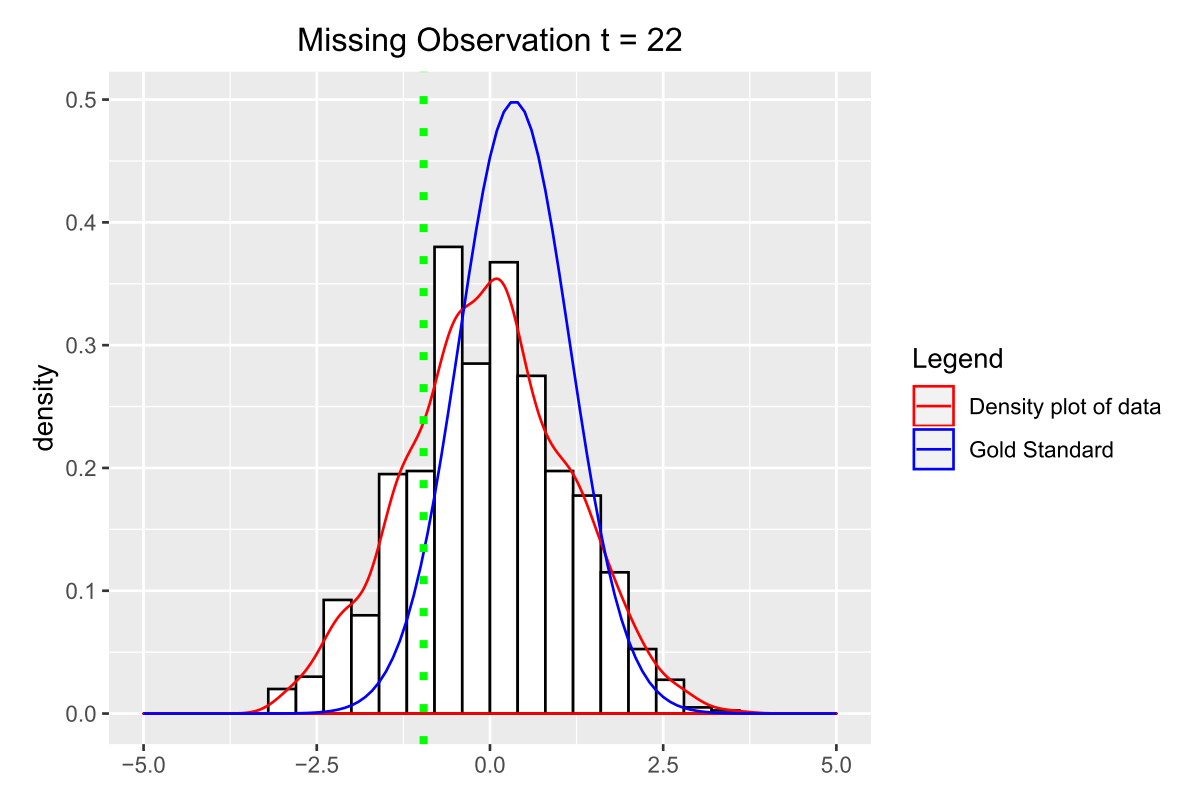
\includegraphics[width=0.5\linewidth]{ar1_001.PNG}}
 \subfloat[fig 2]{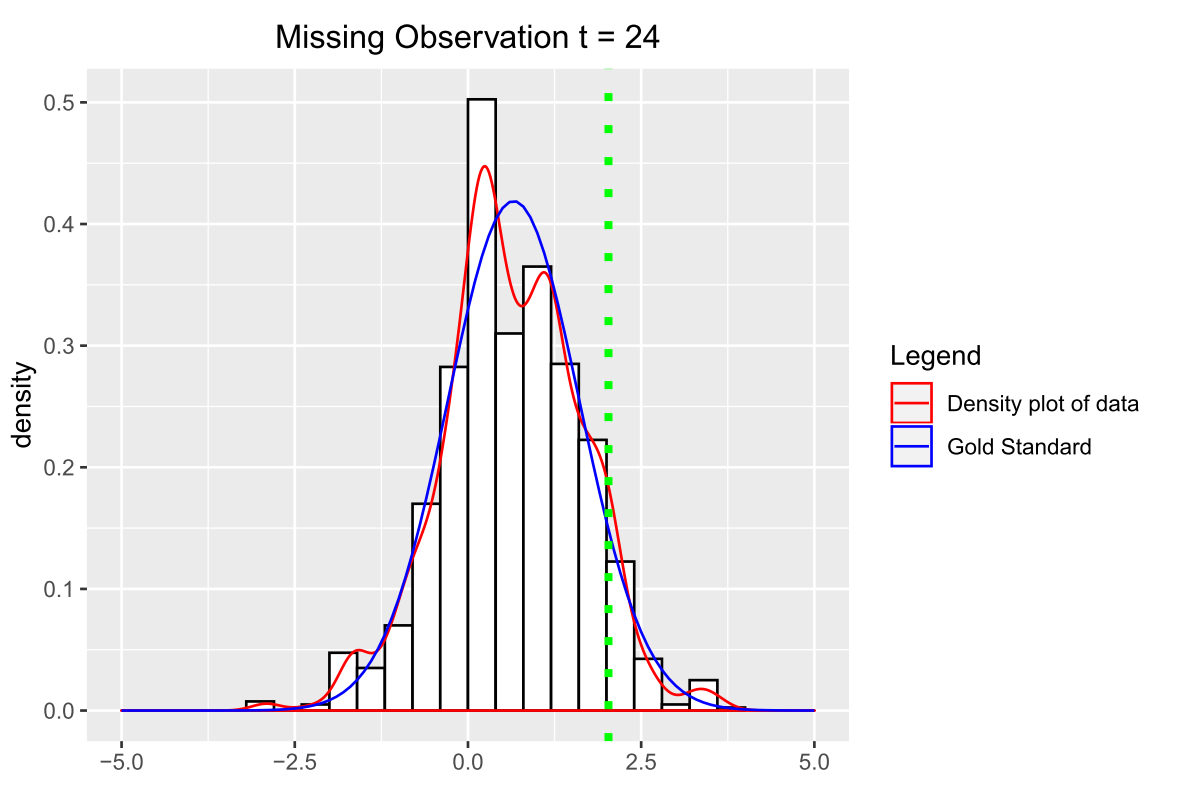
\includegraphics[width=0.5\linewidth]{ar1_002.PNG}}\\
 \subfloat[fig 3]{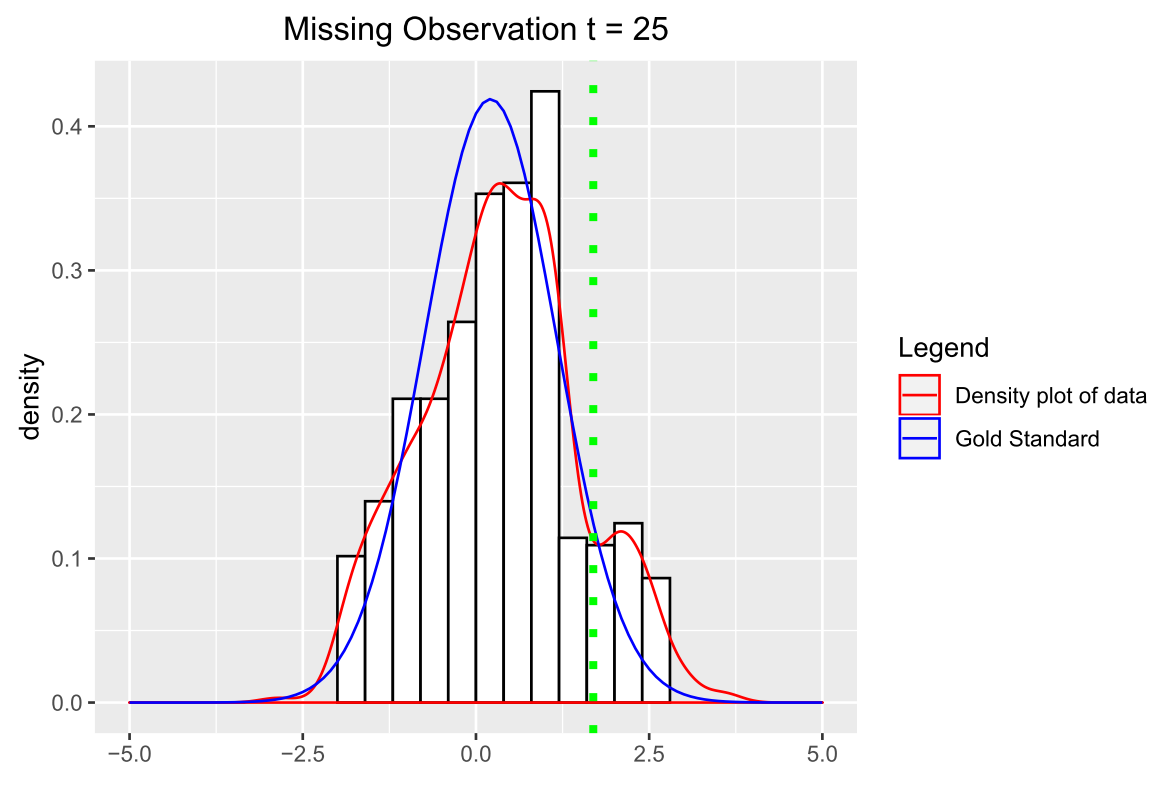
\includegraphics[width=0.5\linewidth]{ar1_003.PNG}}
 \subfloat[fig 4]{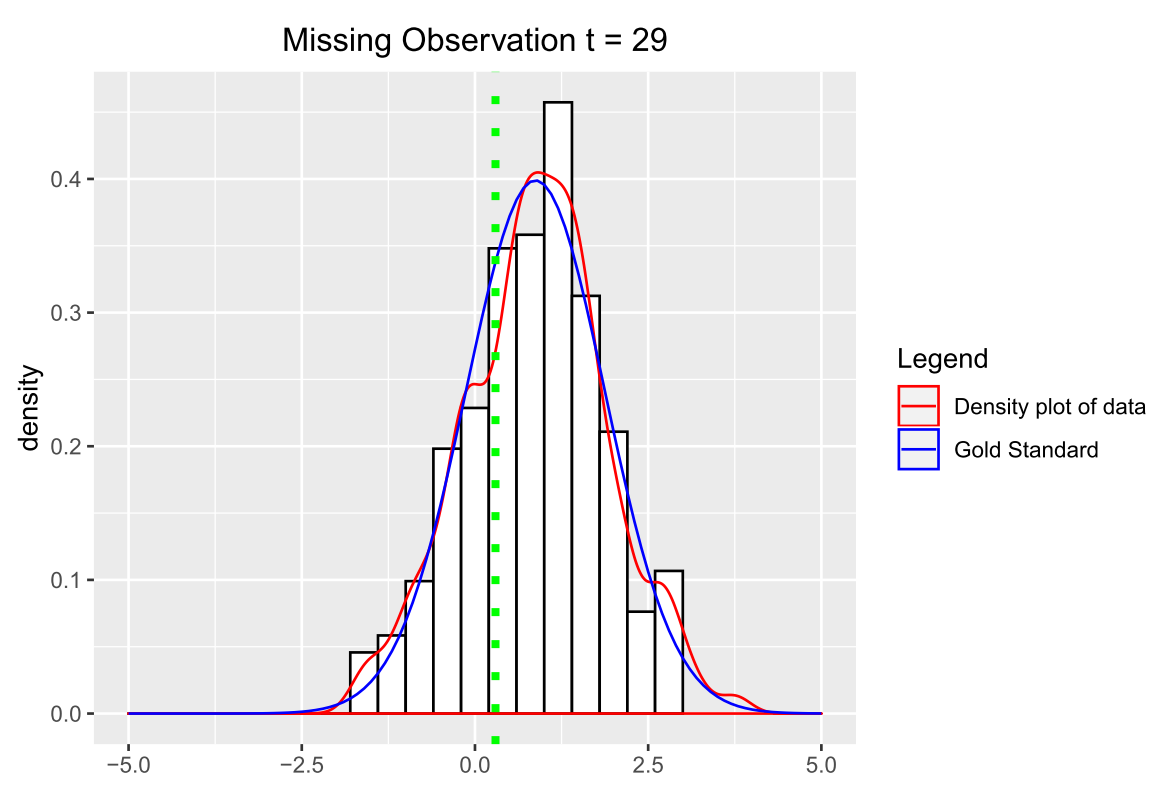
\includegraphics[width=0.5\linewidth]{ar1_004.PNG}}\\
 \subfloat[fig 5]{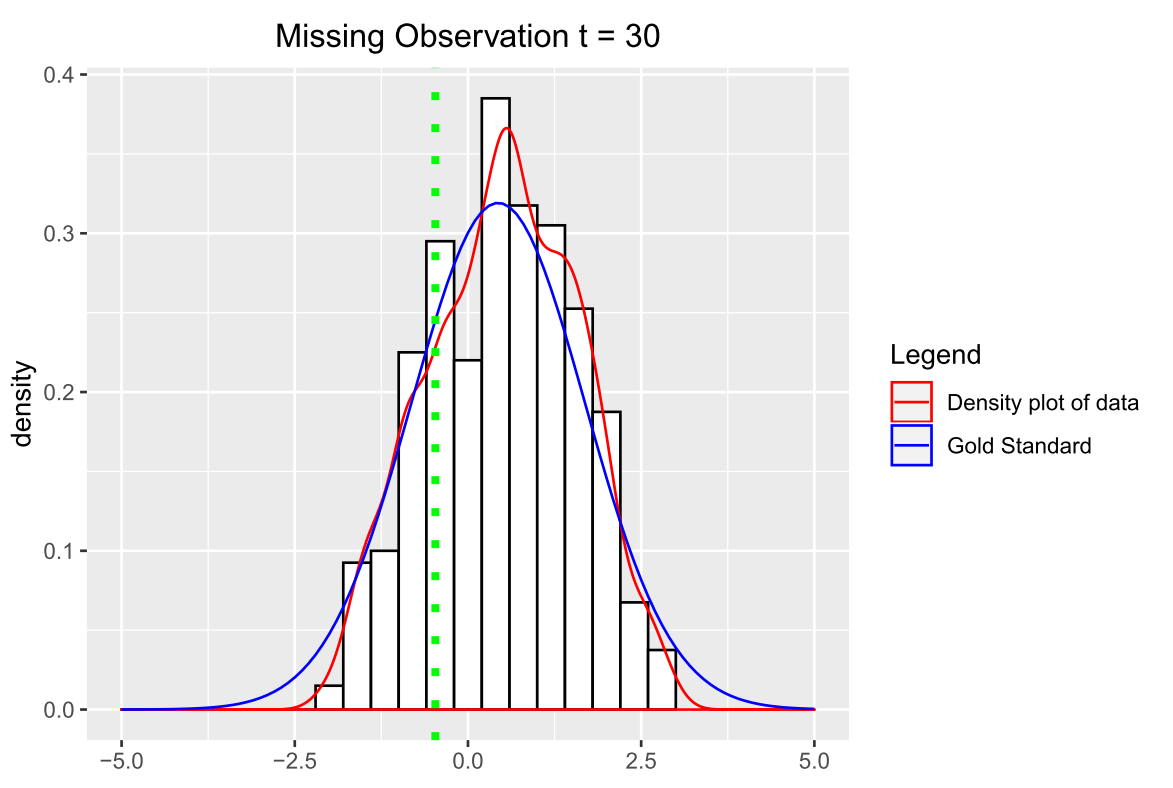
\includegraphics[width=0.5\linewidth]{ar1_005.PNG}}
% figure caption is below the figure
\caption{AR(1) MODEL: Simulations with 1,000 particles and 30 times compared to the gold standard for the 5 missing times of the AR(1) model. In Green the value for the observation. The AR(1) model had parameter $\varphi = 0.5$, variance $\sigma^2 = 1$. The Bernoulli distribution had parameter $p = 0.2$}
\label{fig:1}       % Give a unique label
\end{figure*}
%

\section{Application to the the algae invasion of a river}

This second application of our methodology is an example of how the SIS with correction algorithm can be applied to a real life problem. 

In this example we are going to consider a river infested by some form of alien algae. We will consider the river as one dimensional as the expansion of the invasion will happen along the length of the river. For simplicity we will consider the section of a river without tributary or confluences. 

We will divide the length of the river in $N$ sections or cells and we will consider the first invasion to start in the cell with index $m$.
From the cell indexed by $m$ the invasion can propagate only in the immediately adjacent section of the river, namely the cells indexed by $m-1$ and $m+1$, with probability $\theta$. Following this rule we introduce the binary vectors $\vec{x}^{i} = (x_1^{i}, \dots, x_{N}^{i})$ of the state of the invasion at time $i = 1, \dots, t$. These vectors will all have length $N$, and their elements will define the state of each cell at time $i$: 1 if the cell is invaded and 0 if the cell has not been invaded yet. The invasion will be complete, and all the cells will be invaded, at an unknown time $T$. 
The invasion will expand in two directions (left and right) and the elements of the vector $\vec{x}$ that are adjacent to an infested cell on the right and on the left will have the same probability $\theta$ of being invaded. These vectors will define a $t\times N$ matrix $\vec{X}^{t}$, in which each row $i$ is a vector $\vec{x}^{i}$

We will store the information about the cells that have been observed at or before time $i = 1, \dots, t$ in binary vectors $\vec{z}^{i} = (z_1^{i}, \dots, z_{N}^{i})$, where $z_s^{i} = 1$ if $x_s^{i} = 1$ and the invasive species has been detected at location $s$ at or before time $i$, and $z_s^{i} = 0$ otherwise. As for the AR(1) model example, once a cell has been observed it will remain observed at all subsequent times, therefore if $z_s^{i} = 1$ at time $i$, then we must also have $z_s^{i^{*}} = 1$ at all subsequent times $i^{*} > i$. These vectors will define a $t \times N$ matrix $\vec{Z}^{t}$, in which each row $i$ is a vector $\vec{z}^{i}$.

We will model the new observations on the left and on the right of the previously observed nests in two ways: Firstly, we will consider observations made by a a probe that will check each unobserved cell in sequence. For example, if a cell is observed as invaded at time $t-1$, at time $t$ the probe will start checking the adjacent cell for which we previously did not detect any invader. If that cell is invaded and observed, the probe will proceed to check the subsequent section and so on until there will be a cell where the probe cannot find any invader. The probe might or might not be able to observe the invasion as the algae might not be easy to detect, and will stop searching when it will find the first uninvaded cell. The probability of observing a cell as invaded will be $\theta$.

We will then model the observations as if done randomly by the population reporting on the invasion. In this case, the invaded cells will all have the same probability $\theta'$ of being observed. Notice that we will have observations in cells that are not adjacent to a previously observed one. When this happens, all the uninvaded cells between the newly observed one and the one observed at time $t-1$ will be automatically considered as invaded.

In this example, as for the AR(1) model, our observations are going to be deterministic.

\subsection{Bayesian inference in a partially observed state space}

We want to determine the posterior distribution in light of observations $p(\vec{X}^{t} | \vec{Z}^{t})$ and this is obtained, as for the AR(1) model, renormalising the prior at time $t$, $q(\vec{X}^{t}, \vec{z}^{t} | \vec{Z}^{t-1})$, over values consistent with the observations $\vec{Z}^{t}$.

\[
    p(\vec{X}^{t} | \vec{Z}^{t})  =  \frac{q(\vec{X}^{t}, \vec{z}^{t} | \vec{Z}^{t-1})}{r(\vec{z}^{t} | \vec{Z}^{t-1})}
\]
where 
\[
    r(\vec{z}^{t} | \vec{Z}^{t-1}) = \sum_{x_s^{t}} q(\vec{X}^{t}, \vec{z}^{t} | \vec{Z}^{t-1}).
\]
for $s = 0, \dots, N$ such that $z_s^{t}=0$.

The prior for time $t$, $q(\vec{X}^{t}, \vec{z}^t | \vec{Z}^{t-1})$ represents our knowledge about the state before we observe $\vec{z}^{t}$ and can be written as:
\begin{align}
    & q(\vec{X}^{t}, \vec{z}^{t} | \vec{Z}^{t-1}) = p(\vec{z}^{t} | \vec{X}^{t}, \vec{Z}^{t-1}) p(\vec{x}^{t} | \vec{X}^{t-1}) p(\vec{X}^{t-1} | \vec{Z}^{t-1}) \label{eq:3}
\end{align}
Since the process $x$ does not depend on the observations, so $p(\vec{x}^{t} | \vec{X}^{t-1}, \vec{Z}^{t-1}) = p(\vec{x}^{t} | \vec{X}^{t-1})$.

The distribution for the observations will be:
\begin{align*}
    & p(\vec{z}^{t} | \vec{X}^{t}, \vec{Z}^{t-1}) = p(\vec{z}^{t} | \vec{x}^{t}, \vec{z}^{t-1}) \\
    & = p_R(\vec{z}^{t} | \vec{x}^{t}, \vec{z}^{t-1}) p_L(\vec{z}^{t} | \vec{x}^{t}, \vec{z}^{t-1})
\end{align*}
where $p_R(\vec{z}^{t} | \vec{x}^{t}, \vec{z}^{t-1})$ is the probability of the new detections on the right of the cells previously observed invaded and $p_L(\vec{z}^{t} | \vec{x}^{t}, \vec{z}^{t-1})$ is the probability of the new detections on the left of the cells previously observed invaded. These two processes are independent.

Let $a^{t}$ be the largest integer in the set $\{ s : z_s^{t} = 1 \}$, that is, the index of the highest numbered cell at which the invader has been observed at time $t$ on the right of the invasion. Then the number of new probes at which the invader is successfully detected at time $t$ is $a^{t} - a^{t-1}$. Probing on the right can stop in two ways: either because all invaded sites on the right have been found, in which case $p_R(\vec{z}^{t} | \vec{x}^{t}, \vec{z}^{t-1}) = \varphi^{a^{t} - a^{t-1}}$, or because the last probe on the right failed to detect an invaded cell, in which case $p_R(\vec{z}^{t} | \vec{x}^{t}, \vec{z}^{t-1}) = \varphi^{a^{t} - a^{t-1}} (1 - \varphi)$.

Similarly, let now $c^{t}$ be the smallest integer in the set $\{ s : z_s^{t} = 1 \}$, that is, the index of the smallest cell at which the invader has been observed at time $t$ on the left of the invasion. Then the number of new probes at which the invader is successfully detected at time $t$ is $c^{t} - c^{t-1}$.

The distribution for the observation will therefore be:
\begin{align*}
    p(\vec{z}^{t} | \vec{x}^{t}, \vec{z}^{t-1}) = &\varphi^{(a^{t} - a^{t-1})} \bigg(1 - \varphi \bigg)^{1-\one {a^{t}=\gamma^{t}}}\\
    &\varphi^{(c^{t} - c^{t-1})} \bigg( 1 - \varphi \bigg)^{1-\one {c^{t}=\beta^{t}}}
\end{align*}
were $\gamma^{(t)}$ is the limit of the invasion on the right and $\beta^{(t)}$ is the limit of the invasion on the left.
Notice that for simplicity we will assume that we observe the beginning of the invasion at time $t=1$. 

The distribution for the invasion if the expansion can happen in two directions is:
\begin{equation*}
    p(\vec{x}^{t} | \vec{X}^{t-1}) = p(\vec{x}^{t} | \vec{x}^{t-1}) = p_R(\vec{x}^{t} | \vec{x}^{t-1}) p_L(\vec{x}^{t} | \vec{x}^{t-1}) 
\end{equation*}
separating the expansion on the left and on the right of the invasion.
These two expansions are independent. Then, $p_R(\vec{x}^{t} | \vec{x}^{t-1}) = \theta$ if the invasion has expanded one cell to the right, and $p_R(\vec{x}^{t} | \vec{x}^{t-1}) = 1 - \theta$ if no expansion to the right has occurred, and it's 0 for any other $\vec{x}^{t}$. The same applies to the expansion on the left.

Therefore,
\begin{align*}
       p(\vec{x}^{t} | \vec{X}^{t-1}) &= p_R(\vec{x}^{t} | \vec{x}^{t-1}) p_L(\vec{x}^{t} | \vec{x}^{t-1})\\
       & = \theta^{k} (1-\theta)^{1-k}\theta^{h} (1-\theta)^{1-h} 
\end{align*}
with $k=\{0,1\}$ and $h=\{0,1\}$

Substituting and expanding the recursion in equation \eqref{eq:3} we have
\begin{align*}
        & q(\vec{X}^{t},\vec{z}^{t} | \vec{Z}^{t-1}) = \alpha \prod_{i=2}^{t} \varphi^{(a^{i} - a^{i-1})}\bigg(1 - \varphi \bigg)^{1-\one {a^i=\gamma^i}} \\
        & \varphi^{(c^{i} - c^{i-1})} \bigg(1 - \varphi\bigg)^{1-\one {c^i=\beta^i}} \prod_{i=2}^{r-1} \theta^{k_i} (1-\theta)^{1-k_i} \\ 
        & \prod_{i=2}^{l-1} \theta^{h_i} (1-\theta)^{1-h_i}
\end{align*}
where $l$ is the time where the invasion has reached the end of the river on the left, $r$ is the time where the invasion has reached the end of river on the right, and $\alpha$ is the constant of normalization that will cancel out when at the calculation of the weights.

Similarly to the AR(1) model, since our corrections are deterministic, the unnormalised weights are calculated as follows:
\[
    w^{t_j} = \frac{q(\vec{X'}^{t},\vec{z'}^{t} | \vec{Z}^{t-1})}{q(\vec{X}^{t},\vec{z}^{t} | \vec{Z}^{t-1})}
\]
where the primed are the corrected terms. Again, we will have many cancellations in the calculations of the weights.


% For two-column wide figures use
\begin{figure*}
% Use the relevant command to insert your figure file.
% For example, with the graphicx package use
  \includegraphics[width=\textwidth]{river_007.png}
% figure caption is below the figure
\caption{RIVER INVASION: Simulations with 1,000 particles and 50 cells of 3 possible river invasions all with probability of invasion $\theta = 0.3$ but with different values of the parameter $\varphi$ for the probability of the observations. Figures A1, B1 and C1 show the simulations of the 3 invasions while figures A2, B2 and C2 show the same simulations but with the observations superimposed in red. A1 and A2 show the invasion with $\varphi = 0.3$, B1 and B2 show the invasion with $\varphi = 0.1$. Figure C1 and C2 show the invasion with $\varphi = 0.8$.}
\label{fig:2}       % Give a unique label
\end{figure*}
%
\section{Conclusions}

(HHH to be finalised).

%\section{Section title}
%\label{sec:1}
%Text
%\subsection{Subsection title}
%\label{sec:2}
%as required. Don't forget to give each section
%and subsection a unique label (see Sect.~\ref{sec:1}).
%\paragraph{Paragraph headings} Use paragraph headings as needed.
%\begin{equation}
%a^2+b^2=c^2
%\end{equation}

% For one-column wide figures use
%\begin{figure}
% Use the relevant command to insert your figure file.
% For example, with the graphicx package use
%  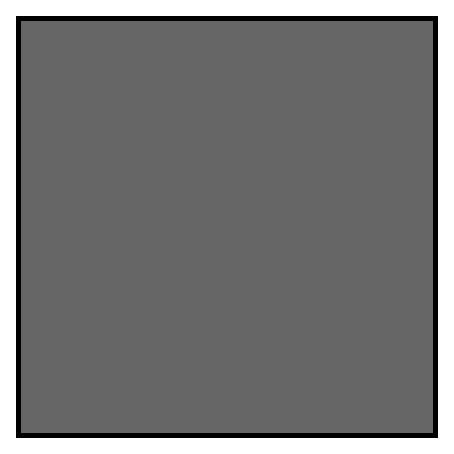
\includegraphics{example.eps}
% figure caption is below the figure
%\caption{Please write your figure caption here}
%\label{fig:1}       % Give a unique label
%\end{figure}
%
% For two-column wide figures use
%\begin{figure*}
% Use the relevant command to insert your figure file.
% For example, with the graphicx package use
%  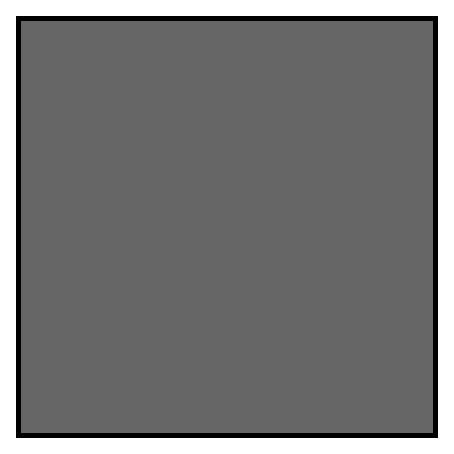
\includegraphics[width=0.75\textwidth]{example.eps}
% figure caption is below the figure
%\caption{Please write your figure caption here}
%\label{fig:2}       % Give a unique label
%\end{figure*}
%
% For tables use
%\begin{table}
% table caption is above the table
%\caption{Please write your table caption here}
%\label{tab:1}       % Give a unique label
% For LaTeX tables use
%\begin{tabular}{lll}
%\hline\noalign{\smallskip}
%first & second & third  \\
%\noalign{\smallskip}\hline\noalign{\smallskip}
%number & number & number \\
%number & number & number \\
%\noalign{\smallskip}\hline
%\end{tabular}
%\end{table}


%\begin{acknowledgements}
%If you'd like to thank anyone, place your comments here
%and remove the percent signs.
%\end{acknowledgements}

\begin{thebibliography}{}

\bibitem [\protect\citeauthoryear{Beer}{1990}]{Beer} 
Beer, T.: The Australian National Bushfire model project. Math Comput. Model. 13(12), 49-56 (1990)

\bibitem [\protect\citeauthoryear{Del Moral}{2014}]{Del Moral} 
Del Moral, P., Murraly, L.M.: Sequential Monte Carlo with Highly Informative Observations. Math Comput. Model. 13(12), 49-56 (1990)

\bibitem [\protect\citeauthoryear{Malathy}{2011}]{Malathy} 
Malathy, A., Baboo, S.S.: An Enhanced Algorithm to Predict a Future Crime using Data Mining. Int. J. Comput. Appl. 21(1), 1-6 (2011)

\bibitem [\protect\citeauthoryear{Nakagawa}{2015}]{Nakagawa}
Nakagawa, S.: Missing data. In: Fox G.A., Negrete-Yankelevich S., Sosa V.J. (eds.) Ecological Statistics: Contemporary theory and application, pp 81-105. Oxford University Press (2015). 

\bibitem[\protect\citeauthoryear{O'Neill}{2002}]{O'Neill}
O'Neill, P.D., Roberts G.O.: Bayesian inference for partially observed stochastic epidemics. J. R. Stat. Soc. A. Stat. 162(1), 121-129 (2002)

\bibitem [\protect\citeauthoryear{Rubin}{1987}]{RubinMI}
Rubin, D.B.: Multiple imputation for nonresponse in surveys. Wiley, New York (1987)

\bibitem [\protect\citeauthoryear{Rubin}{1987}]{Rubin}
Rubin, D.B.: The Calculation of Posterior Distributions by Data Augmentation: Comment: A Noniterative Sampling/Importance Resampling Alternative to the Data Augmentation Algorithm for Creating a Few Imputations When Fractions of Missing Information Are Modest: The SIR Algorithm. J. Am. Stat. Assoc. 82(398), 543-546 (1987)

\bibitem [\protect\citeauthoryear{Tanner and Wong}{1987}]{Tanner}
Tanner, M.A., Wong, W.H.: The Calculation of Posterior Distributions by Data Augmentation. J. Am. Stat. Assoc. 82(398), 528-540 (1987)

\bibitem [\protect\citeauthoryear{Zhang}{2015}]{Zhang}
Zhang, X-P. et al.: Multiple Imputations Particle Filters: Convergence and Performance Analyses for Nonlinear State Estimation with Missing Data. IEEE J. Sel. Top Signa. 9(8), 1536-1547 (2015)

\end{thebibliography}
\end{document}

